\documentclass[12pt, right open]{memoir}
\usepackage{graphicx}
\usepackage{tikz}
\usetikzlibrary{matrix,chains,positioning,decorations.pathreplacing,arrows,automata}
\usetikzlibrary{shapes.geometric, calc, intersections}
\usepackage{mathtools}
\usepackage{amsmath}
\usepackage{float}
\floatstyle{boxed}
\restylefloat{figure}

\graphicspath{data/images}

\usepackage{ifthen}
\setcounter{secnumdepth}{5}


\begin{document}
\chapter{Introduction}
The whole universe is seen in the form of a person. The body of the universe consists of the 12 Rashis, which can be roughly translated as “astrological signs.” Each Rashi represents a part of the body. The nine Grahas or planets govern this universal body. The 12 Rashis are represented in the Maharishi Jyotish program as 12 equal segments of a circle, each covering 30 degrees.The sequence of the 12 Rashis begins with Mesha as the first Rashi.

\begin{figure}
\centering
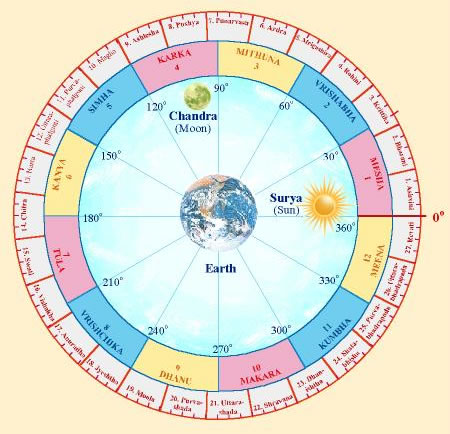
\includegraphics[scale=1]{data/images/jyotish_nakshatras.jpg}
\caption{The Circle of 27 Nakshatras with Reference to the Earth}
\end{figure}

This illustration shows the sequence of the 27 equal segments of the Nakshatras, each consisting of 13 degrees 20 minutes, with their Sanskrit names and numbers. As seen from the earth, the moon passes through this circle of the 27 Nakshatras in about 27 days. Thus it takes the moon about one day to pass through one Nakshatra. The moon is shown here moving through Pushya Nakshatra in Karka Rashi. This example also shows the sun moving through Ashvini Nakshatra in Mesha Rashi. Each of the other planets are also moving through the 27 Nakshatras.
Nakshatra Pada: Each Nakshatra is divided into 4 equal parts of 3 degrees 20 minutes each part. They are called Nakshatra Pada 1, 2, 3, and 4. Each Nakshatra Pada has its own significance for interpretation.

%\begin{tabular}{|l | l|}
%\hline
%\textbf{Vedic Name} & \textbf{English Names} \\ \hline
% Mesha & Aries \\ \hline
% Vrishabha & Taurus\\ \hline
% Mithuna & Gemini\\ \hline
% Karka & Cancer\\ \hline
% Simha & Leo\\ \hline
% Kanya & Virgo\\ \hline
% Tula & Libra\\ \hline
% Vrishchika & Scorpio\\ \hline
% Dhanu & Sagittarius\\ \hline
% Makara & Capricorn\\ \hline
% Kumbha & Aquarius\\ \hline
% Meena & Pisces\\ \hline
%\end{tabular}

\section{Ashwini Star or Nakshatra}

You are born when the Moon was in Ashwini star or nakshatra. You are Scrupulous, prosperous, obedient, truthful and obtain all comforts. You are endowed with good family and children and wealth. You are daring, handsome and monied. You are a capable administrator, cruel, of big body and respected. You sacrifice money, have a good conduct and an enjoyer. You are quick and candid, a knower of scriputures, rational and succeed in quarrels. You have long hands and wide eyes. You are respected by Kings and governments and speak sweetly. You are daring, arrogant, thief and a fraud. You are unkind, practice of forbidden paths, intelligent and contain some sympal on your girdle. You are fickle and undertake travelling. You may court other women and are farsighted. You are not independent, but strong.


\section{Bharani Star or Nakshatra}

If you are born in Bharani Star, incur the displeasure of others, enjoyer, obedient and learned, fear water and get the wealth of bad people. You know the scriptures, rationale, intelligent and win the quarrels. You bear scars on your body due to injuries. You are good speaker and suffer from heart diseases. You are stable, knowledgeable and truthful. You are longlived. You are also determined, and proud, you do not tolerate other’s prosperity.


\section{Krithika Star or Nakshatra}

If you are born with Krithika star, benefit of friends and family, endowed with son and enjoy life and are very prosperous. You suffer from hunger and are without strength and money, you undertake purposeless travelling but recollect the help rendered by others. You are very harsh and do jobs forbidden. You are cruel and do good jobs and they also have defective face. You are bright, instant angry and run after other women. You are heavy eater and fiery. You are stingy, intelligent, famous, successful, loved by partner, with property earned by yourself, white haired, afraid of wind, and carry the symbols of til and fish.


\section{Rohini Star or Nakshatra}

If you are born with Rohini Star, you are agriculturist, expert, well behaved, handsome, good speaker and poet. You are stable minded, respected, enjoyer and interested in love making. You are of sweet speech, intelligent, capable and bright. You are longlived and perform accepted jobs, religious, truthful and help those who have helped you. You are respected by government. You respect Gods and Brahmins and know the science of metres and metaphors. You are able servants of your lord and determined. You are endowed with good looking hands and wide forehead, handsome, independent, loved by your children, experts, wealthy and respect to corns and money, have desire to wear new clothes, suffer from eye diseases, litter feared and play with women.


\section{Mrigashira Star or Nakshatra}

If you are born with Mrigashira or Mrigaseesha Star, you are truthful, handsome, enjoywealth and prosperity, pure in heart, bright, sage like and fickle minded. You are interested in learning, obedient, always loving teachers, friendly with government authorities and respected by them. You are enthusiastic, feared, monied, lovable, knowledgeable in architecture, kingly and good administration. You are pleasant spoken, intelligent and affectionate to your mother. You are quick and arrogant and hate others.


\section{Aridhra Star or Nakshatra}

If you are born with Aridhra or Thiruvadhirai Star, you are soft, stable minded, strong, earning by sacrifice, afflicted by sickness, fear and angry. You suffer due to hunger, hard bodied, lovable, forget to help rendered by others, expert in trade and commerce, cruel, having may relatives, ill advisers and hate all. You are with pride, of lower levels and do jobs which are forebidden. You are benefit of money and corns. Such people are poets, little learned, longlived and little interested in things.


\section{Punarvasu or Punarpoosam Star}

You are endowed with children, good qualities, wealth and you indulge in bringing difference of opinion among friends. You speak very clearly and are secretive in your dealings. You are learned in the sciences and interested in personal decoration of gems and gold ornaments. You are givers and famous. You are religious, attractive, carry out works of other women. You are tolerant, satisfied with small things and fast moves. You collect a good circle of friends, daily eat good food, sacrificer and worship lord Vishnu. You are peaceful, happy, enjoying a endowed with good progeny. You are noted to be longlived, loved by wife, handsome, interested in pomp, of good heart, high in conduct, with low voice, like cereals, intelligent, thinker and possess fish sign on stomach.


\section{Pushya or Poosam Star}

You are wealthy, happy, respected, stable minded, endowed with handsome body, respecting parent, following their religion and most obedient. You command money and vehicles of novelty. You are important person in the world, knowledgeable in the science of spells and respected by government.You retain your stand, and are happy. You are characterized by the presence of fish symbol on the hands and feet,. You are endowed with all good qualities, short tempered and interested in the discussion of scriptures.


\section{Ashlesha or Oilyam Star}

You are cruel, daring and angry, you probably co-habit with people of same sex and animals like cow. You travel aimlessly, do undesirable jobs, harmful to your own and other people, you are proud, and suffer on a account of sex starvation. You are angry and are strong like lion. You know Brahman and dependent on others for life. You are cruel to all beings, pay fines by doing sinful acts, unstable minded and fearful. You are always sad, serve others, short tempered and vary bad persons. You are childish, slow in the work of your lord, wide eyed, endowed with fish sign in eyes, develop enmity with your own people, highly stingy and stubborn.


\section{Magham or Magha Star or Nakshatra}

You are reserved, highly sexy, endowed with comforts and have wife who are also reserved, knowledgeable, pure and sacrifice things. You are cruel, respect your father, sharp in reacting with others, non-sinners and destroy your enemies. You are harsh spoken, hefty bodies, angry, transact with teachers and government, interested in the advise of well wishers or sages and are bright. You tread the religious path and endowed with pleasant qualities, enjoyer and truthful. You are served by many servants, conduct big operations and are leader of a big party or army. You are learned, long lived, earn good money, obedient and help your relatives. You have blood shot eye and possess fish sign on the chest.


\section{Poorvaphalguni or Pooram Star or Nakshatra}

You are expert in love making, strong and handsome, but extremely fearful. You help others, and carryout works which cannot be done by others. You are angry, fraud, cruel and candid. You are bright, wealthy, giver, expert in music and dance. You are wise and are in the government service. You are longlived and and be get few children. You are learned, reserved, handsome, love your brothers, endowed with soft hands and feet, born of Rajamsha, strict transactor, endowed with a attractive eyes, idle and possess government signs.


\section{Uttaraphalguni or Utharam Star}

You are wealthy, knowing the science of weapons, impotent, respectful and endowed with attractive eyes. You are fixed to the scienes and stingy in spending money. You are giver, kind hearted, happy and endowed with good qualities, famous, kingly, daring and extremely soft personalities. You win over your enemies, loved by women, experts in arts, truthful and learned. You are obedient, religious, loved by people, stable and bright. You are fearful and good warmers.


\section{Hastham or Hastha Star or Nakshatra}

You are stable bodied, untruthful, bear excellent character and warrior. You are giver, independent, famous, interested in worshipping of gods and pious people, and likely to get all the properties of your father. You are learned, handsome, wealthy, daring, helpful to others and all knowledgeable. You are cruel and grab other’s property. You are bad people, strong, interested in music, happy with your relatives and friends, respected by government authorities, respect the gods and pious, destroy your enemies, famous and possess the signs of fish.


\section{Chitra Star or Nakshatra}

Those born in their star Chitra, are extremely fearful of low mind suffer from hunder, and troubled in mind. They are weak and perverse sexed. They are troubled by their enemies, obedient, capable and wear peculiar dresses. They advance peculiar arguments. They are experts in love making, bright, wealthy, enjoyers and learned. They are probably distorted (personalities), strong, brave, endowed with wife and children and respect the gods and pious.


\section{Swati Star or Nakshatra}

Those born in Swati star, are wise, witty and learned. They are religious and pleasant minded. They are endowed with the body of kingly symbols, bright and handsome and loved by their wives. They perform religious works, truthful, expert in transactions, sexy, givers and learned. They are obedient, lovers of pious people, experts in architecture and sculpture, stingly and respect gods and Brahmins. They help others, daring, long lived, large eyed, kind, famous, lover of relatives and friends, independent, eat optimum food, and followers of their own religion.


\section{Vishaka Star or Nakshatra}

Those born in Vishaka star are physically impure, strong, go after other’ women, benefit of relatives, and cause deference among friends. They are always thinking about sex, experts in the jobs of fire, brewery, lores and metallurgical operations and do not develop friendship with any body. They are jealous, subile, kind, forbidden love, of controlled senses, wealthy and stingy. They are intelligent, stable minded, good speakers, love relatives, children and friends. They are great people. They are candid quarrel some and addicted to prostitutes. They are witty, obedient, long lived, help many, speakers of truth, short tempered, lovers of women, possess blood shot eyes and also fish sign on the secret parts.


\section{Anuradha or Anusha Star or Nakshatra}

Those born in the star Anuradha are interested in women with commandable complexion of the boday, be wildered, idle and weak minded. They are famous, experts in arts, and destroyers of their enemies. They are servers of Government, brave, stationed in countries other than their own, handsome, and destroyers of their sins. They are truthful, respect kings, respect their mothers and are musicians. They enjoy life and go after other women. They are fit for friendship, kind hearted, of helping nature, intelligent, enjoyers and travelers.


\section{Jyeshtha or Kettai Star or Nakshatra}

Those born in this Jyeshtha star, are fond of daily physical exercise, warriours, always respecting elders, famous and endowed with fine qualities. They gain fame, are bright, accompany Government, affected in mind, deeply idle, well known and speak final. They are addicted to bad jobs, capable of underging difficulties, unbearable, cruel, untruthful and wealthy, they are tall and endowed with few children.


\section{Moola Star or Nakshatra}

Those born in moola star, are fast workers, soft, fickle, endowed with good qualities, harmful and untrustworthy. They route out the different parties unconcerned, otherwise they enhance the prosperity of their clean and comfort their mothers. They are sagelike, wealthy, enjoyers, helping others, comforted by women and suffer from phlegm diseases. They are also proud, serve the government, processes knowledge of finer aspects, daily enjoyers, handsome and hated by all. They are happy and have vehicles, harmful, do permanent jobs, and famous by defeating their enemies. They are religious, thieves, respectable, show affection to relatives, red complexioned, sexy, obedient, independent, blood shot-eyed and loved by women.


\section{Purvashadha or Pooradam Star or Nakshatra}

Those born in this purvashadha Star, are thieves, proud, angry, wealthy, endowed with good qualities, always speak untruth and capable. They are drunkards, fickle, good speakers, having attractive face, obedient, lovers of cows, suffer ungrudgingly, youthful and live with respect. They help at the sight of difficulty, loved by people and experts in almost all fields. They are slightly taller, possess sublet fingures, famous sophisticated.


\section{Uttarashadha or Uthiradam Star or Nakshatra}

Those born in this uttarashadha star are born with Brahamsa, cause difference of opinion between friends, do physical exercises, loved by people, enjoyers and travel a lot. They are givers, successful, obtain enjoyment from wife and happy. They recollect the help rendered by others, religious, obedient, handsome and wealthy. Loved by their relatives they are great givers. They are all knowledgeable, pure, endowed with good qualities, entertain guests, witty, kind hearted, furnished of grand qualities, brave, endowed with long nose and fish signs and private parts.


\section{Shervana or Thiruvonam Star or Nakshatra}

Those born in this Shravana Star are experts in music, dance and drama, truthful and stable minded, they enjoy hearing scriptures. They are endowed with many children and friends, respect pious people, win over their enemies, large-hearted, knowledgeable, brave, learned, wealthy, expert in arts, religious, famous, givers, recollect the help rendered by others, accompanied by relatives, and pure in heart. They are interested in scents and flowers, hefty bodied, go after other women, handsome, large hearted, support many relatives and loved by all. They are good, speakers, enjoy life, wise, possess signs of fish on private parts.


\section{Dhanishta or Avittam Star or Nakshatra}

Those born in Dhanishta star are difficult to win, benefit of sadness, good eaters and very famous. They serve the elders and always protect others. They are religious, endowed with many good qualities, wealthy, kind hearted and having good establishment. They are sad, cruel, suffer from disease like tuberclosis, and are stubborn. They are after other women, daring and loved by women. They worship the god and elders, good givers and wealthy. They are interested in music, respected by relatives, decorated by jewellery and rule many people. They are bright, jobfull, cruel, hate Brahmins, hot constitutional, stingy and possess long feet. They speak much and show pride in undertaking many works.


\section{Shatabhisha or Sathayam Star or Nakshatra}

Those born in this Shatabhisha star are endowed with many children, angry, daring, extreme and unbearable; they are almost selfish and gamblers. They are of questionable character and experts in magic. They are stubborn, stable minded, specially knowledgeable, brave, cruel, eat little, stingy, wealthy, servers and go after other women. They live in foreign lands and most sexy, they are respected by the world, plenty minded, their enemies, long lived and are witty. They are good in various transactions, astrologers, suffer from various diseases and are endowed with some knowledge.


\section{Purvabhadra or Poorattathy Star or Nakshatra}

Those born in this Purvabhadra Star, and worship of gods and teachers, of righteous conduct and of broad minded. They are respectable and above controversies. They are having control over their senses, experts in all kinds of jobs, endowed with good chest, they are at home with the learned, determined, won over by women, stubborn, despire others, irreligious, brave, givers, enjoyers, soft spoken, handsome and living their relatives. They are speakers, endowed with children, help excess, possess long tongue, suffer from the disease of ears, obedient, helping nature.


\section{Uttarabhadra or Uthirattathy Star or Nakshatra}

Those born in this Uttorabhadra Star suffer from fluctuation of funds, wise and surrounded by many people. They are affected by the imbalance of bile and always ride. They are prominent among their clan, wear jewels, always do constructive jobs, obtain wealth, and cors and they are givers. They are endowed with children, religious, winners of their enemies, happy, determined, sexy, learned, sacrificers, respected in all circles, suffer ferom various diseases, brave, wise, idle, fickle, possess the signs of fish an til on their private parts and loved by their relatives. They are just and they earn by righteous means.


\section{Revathi Star or Nakshatra}

Those born in this Revathi Star practice intelligent things, candid, handsome, talk angrily and quick. They are independent in pursuing any jobs. They are endowed with good qualities, have control over their senses, always thinking about their home, wise, handsome, wealthy, enjoy life, learned, fickle, earn good money, sexy, brave, givers, lose women, pure in mind, endowed with well proportioned body, capable, hefty bodied, bright, help others and move foreign lands.


\end{document}